% Options for packages loaded elsewhere
\PassOptionsToPackage{unicode}{hyperref}
\PassOptionsToPackage{hyphens}{url}
%
\documentclass[
  12pt,
]{article}
\title{Effective Pest Treament That Protects Pollinators}
\usepackage{etoolbox}
\makeatletter
\providecommand{\subtitle}[1]{% add subtitle to \maketitle
  \apptocmd{\@title}{\par {\large #1 \par}}{}{}
}
\makeatother
\subtitle{\url{https://github.com/shivanikuckreja/CitrolaKuckrejaSaltman_ENV872_EDA_FinalProject/tree/main/Project}}
\author{Sam Saltman, Shivani Kuckreja, Jessica Citrola}
\date{}

\usepackage{amsmath,amssymb}
\usepackage{lmodern}
\usepackage{iftex}
\ifPDFTeX
  \usepackage[T1]{fontenc}
  \usepackage[utf8]{inputenc}
  \usepackage{textcomp} % provide euro and other symbols
\else % if luatex or xetex
  \usepackage{unicode-math}
  \defaultfontfeatures{Scale=MatchLowercase}
  \defaultfontfeatures[\rmfamily]{Ligatures=TeX,Scale=1}
  \setmainfont[]{Times New Roman}
\fi
% Use upquote if available, for straight quotes in verbatim environments
\IfFileExists{upquote.sty}{\usepackage{upquote}}{}
\IfFileExists{microtype.sty}{% use microtype if available
  \usepackage[]{microtype}
  \UseMicrotypeSet[protrusion]{basicmath} % disable protrusion for tt fonts
}{}
\makeatletter
\@ifundefined{KOMAClassName}{% if non-KOMA class
  \IfFileExists{parskip.sty}{%
    \usepackage{parskip}
  }{% else
    \setlength{\parindent}{0pt}
    \setlength{\parskip}{6pt plus 2pt minus 1pt}}
}{% if KOMA class
  \KOMAoptions{parskip=half}}
\makeatother
\usepackage{xcolor}
\IfFileExists{xurl.sty}{\usepackage{xurl}}{} % add URL line breaks if available
\IfFileExists{bookmark.sty}{\usepackage{bookmark}}{\usepackage{hyperref}}
\hypersetup{
  pdftitle={Effective Pest Treament That Protects Pollinators},
  pdfauthor={Sam Saltman, Shivani Kuckreja, Jessica Citrola},
  hidelinks,
  pdfcreator={LaTeX via pandoc}}
\urlstyle{same} % disable monospaced font for URLs
\usepackage[margin=2.54cm]{geometry}
\usepackage{color}
\usepackage{fancyvrb}
\newcommand{\VerbBar}{|}
\newcommand{\VERB}{\Verb[commandchars=\\\{\}]}
\DefineVerbatimEnvironment{Highlighting}{Verbatim}{commandchars=\\\{\}}
% Add ',fontsize=\small' for more characters per line
\usepackage{framed}
\definecolor{shadecolor}{RGB}{248,248,248}
\newenvironment{Shaded}{\begin{snugshade}}{\end{snugshade}}
\newcommand{\AlertTok}[1]{\textcolor[rgb]{0.94,0.16,0.16}{#1}}
\newcommand{\AnnotationTok}[1]{\textcolor[rgb]{0.56,0.35,0.01}{\textbf{\textit{#1}}}}
\newcommand{\AttributeTok}[1]{\textcolor[rgb]{0.77,0.63,0.00}{#1}}
\newcommand{\BaseNTok}[1]{\textcolor[rgb]{0.00,0.00,0.81}{#1}}
\newcommand{\BuiltInTok}[1]{#1}
\newcommand{\CharTok}[1]{\textcolor[rgb]{0.31,0.60,0.02}{#1}}
\newcommand{\CommentTok}[1]{\textcolor[rgb]{0.56,0.35,0.01}{\textit{#1}}}
\newcommand{\CommentVarTok}[1]{\textcolor[rgb]{0.56,0.35,0.01}{\textbf{\textit{#1}}}}
\newcommand{\ConstantTok}[1]{\textcolor[rgb]{0.00,0.00,0.00}{#1}}
\newcommand{\ControlFlowTok}[1]{\textcolor[rgb]{0.13,0.29,0.53}{\textbf{#1}}}
\newcommand{\DataTypeTok}[1]{\textcolor[rgb]{0.13,0.29,0.53}{#1}}
\newcommand{\DecValTok}[1]{\textcolor[rgb]{0.00,0.00,0.81}{#1}}
\newcommand{\DocumentationTok}[1]{\textcolor[rgb]{0.56,0.35,0.01}{\textbf{\textit{#1}}}}
\newcommand{\ErrorTok}[1]{\textcolor[rgb]{0.64,0.00,0.00}{\textbf{#1}}}
\newcommand{\ExtensionTok}[1]{#1}
\newcommand{\FloatTok}[1]{\textcolor[rgb]{0.00,0.00,0.81}{#1}}
\newcommand{\FunctionTok}[1]{\textcolor[rgb]{0.00,0.00,0.00}{#1}}
\newcommand{\ImportTok}[1]{#1}
\newcommand{\InformationTok}[1]{\textcolor[rgb]{0.56,0.35,0.01}{\textbf{\textit{#1}}}}
\newcommand{\KeywordTok}[1]{\textcolor[rgb]{0.13,0.29,0.53}{\textbf{#1}}}
\newcommand{\NormalTok}[1]{#1}
\newcommand{\OperatorTok}[1]{\textcolor[rgb]{0.81,0.36,0.00}{\textbf{#1}}}
\newcommand{\OtherTok}[1]{\textcolor[rgb]{0.56,0.35,0.01}{#1}}
\newcommand{\PreprocessorTok}[1]{\textcolor[rgb]{0.56,0.35,0.01}{\textit{#1}}}
\newcommand{\RegionMarkerTok}[1]{#1}
\newcommand{\SpecialCharTok}[1]{\textcolor[rgb]{0.00,0.00,0.00}{#1}}
\newcommand{\SpecialStringTok}[1]{\textcolor[rgb]{0.31,0.60,0.02}{#1}}
\newcommand{\StringTok}[1]{\textcolor[rgb]{0.31,0.60,0.02}{#1}}
\newcommand{\VariableTok}[1]{\textcolor[rgb]{0.00,0.00,0.00}{#1}}
\newcommand{\VerbatimStringTok}[1]{\textcolor[rgb]{0.31,0.60,0.02}{#1}}
\newcommand{\WarningTok}[1]{\textcolor[rgb]{0.56,0.35,0.01}{\textbf{\textit{#1}}}}
\usepackage{longtable,booktabs,array}
\usepackage{calc} % for calculating minipage widths
% Correct order of tables after \paragraph or \subparagraph
\usepackage{etoolbox}
\makeatletter
\patchcmd\longtable{\par}{\if@noskipsec\mbox{}\fi\par}{}{}
\makeatother
% Allow footnotes in longtable head/foot
\IfFileExists{footnotehyper.sty}{\usepackage{footnotehyper}}{\usepackage{footnote}}
\makesavenoteenv{longtable}
\usepackage{graphicx}
\makeatletter
\def\maxwidth{\ifdim\Gin@nat@width>\linewidth\linewidth\else\Gin@nat@width\fi}
\def\maxheight{\ifdim\Gin@nat@height>\textheight\textheight\else\Gin@nat@height\fi}
\makeatother
% Scale images if necessary, so that they will not overflow the page
% margins by default, and it is still possible to overwrite the defaults
% using explicit options in \includegraphics[width, height, ...]{}
\setkeys{Gin}{width=\maxwidth,height=\maxheight,keepaspectratio}
% Set default figure placement to htbp
\makeatletter
\def\fps@figure{htbp}
\makeatother
\setlength{\emergencystretch}{3em} % prevent overfull lines
\providecommand{\tightlist}{%
  \setlength{\itemsep}{0pt}\setlength{\parskip}{0pt}}
\setcounter{secnumdepth}{5}
\ifLuaTeX
  \usepackage{selnolig}  % disable illegal ligatures
\fi

\begin{document}
\maketitle

\newpage
\tableofcontents 
\newpage
\listoftables 
\newpage
\listoffigures 
\newpage

\hypertarget{rationale-and-research-questions}{%
\section{Rationale and Research
Questions}\label{rationale-and-research-questions}}

\textbf{Pollination is a critical component of agriculture. Honeybees
are important pollinators. Our research looks to see if there are
exposure methods and chemicals that do not cause significant harm to
honeybees while eliminating pests. The goal of our research is to
determine potential treatment methods that reduce pests while having
little to no impact on pollinators.}

Questions:

\begin{enumerate}
\def\labelenumi{\arabic{enumi}.}
\item
  \emph{Is there an exposure type that has less impact on bees than
  non-bee insects?}
\item
  \emph{Are there chemicals that have a high mortality rate for non-bee
  insects and low rate for bees?}
\end{enumerate}

\newpage

\hypertarget{dataset-information}{%
\section{Dataset Information}\label{dataset-information}}

Data Source: The dataset was pulled from a repository created for
Environmental Data Analytics at Duke University in 2020. The data
collected is from several EPA studies on neonicotinoids and their
effects on insects. The data we will be analyzing is the type of
chemical administered, how it was administered, and how both of these
variables affected insects.

In the wrangling process, we selected the relevant information to our
topic. This includes the chemical type, insect species, lifestage and
age of the species, exposure type and the effect of the exposure.

\begin{longtable}[]{@{}
  >{\raggedright\arraybackslash}p{(\columnwidth - 2\tabcolsep) * \real{0.44}}
  >{\raggedright\arraybackslash}p{(\columnwidth - 2\tabcolsep) * \real{0.56}}@{}}
\toprule
\begin{minipage}[b]{\linewidth}\raggedright
Detail
\end{minipage} & \begin{minipage}[b]{\linewidth}\raggedright
Description
\end{minipage} \\
\midrule
\endhead
Data Source & EPA ECOTOX Knowledgebase \\
------- & --------- \\
Retrieved From & \url{https://cfpub.epa.gov/ecotox/help.cfm} \\
------- & --------- \\
Variables Used & Chemical Name, Species Common Name, Organism Lifestage,
Organism Age, Exposure Type, Effect, Effect Measurement \\
------- & --------- \\
Date Range & 1982-2019 \\
\bottomrule
\end{longtable}

\newpage

\hypertarget{exploratory-analysis}{%
\section{Exploratory Analysis}\label{exploratory-analysis}}

\begin{Shaded}
\begin{Highlighting}[]
\NormalTok{Mortality }\OtherTok{\textless{}{-}}\NormalTok{ Processed1\_Filter }\SpecialCharTok{\%\textgreater{}\%}
  \FunctionTok{filter}\NormalTok{(Effect }\SpecialCharTok{==} \StringTok{"Mortality"}\NormalTok{)}

\FunctionTok{kable}\NormalTok{(}\FunctionTok{summary}\NormalTok{(Mortality}\SpecialCharTok{$}\NormalTok{Species.Common.Name), }\AttributeTok{caption =} \StringTok{"Species List"}\NormalTok{)}
\end{Highlighting}
\end{Shaded}

\begin{longtable}[]{@{}lr@{}}
\caption{Species List}\tabularnewline
\toprule
& x \\
\midrule
\endfirsthead
\toprule
& x \\
\midrule
\endhead
Honey Bee & 203 \\
Parasitic Wasp & 165 \\
Italian Honeybee & 91 \\
Asian Lady Beetle & 59 \\
Minute Pirate Bug & 52 \\
Buff Tailed Bumblebee & 47 \\
Parastic Wasp & 41 \\
Carniolan Honey Bee & 29 \\
Braconid Wasp & 26 \\
Sevenspotted Lady Beetle & 25 \\
Bumble Bee & 23 \\
European Dark Bee & 23 \\
Mosquito & 22 \\
Parasitoid & 22 \\
Chalcid Wasp & 20 \\
Stingless Bee & 20 \\
Parasitoid Wasp & 19 \\
Fairyfly Parasitoid & 18 \\
Mulberry Pyralid & 18 \\
Spring Tiphia & 18 \\
Codling Moth & 17 \\
House Fly & 14 \\
Ox Beetle & 14 \\
Japanese Beetle & 13 \\
Predatory Bug & 13 \\
Wireworm & 13 \\
Silkworm & 12 \\
Predatory Mite & 11 \\
Spined Soldier Bug & 11 \\
Vedalia Beetle & 11 \\
Yellow Fever Mosquito & 11 \\
Braconid Parasitoid & 10 \\
Calico Scale & 10 \\
Eastern Subterranean Termite & 10 \\
Glasshouse Potato Wasp & 10 \\
Southern House Mosquito & 10 \\
Two Spotted Lady Beetle & 10 \\
Western Flower Thrips & 10 \\
Convergent Lady Beetle & 9 \\
Mealybug Destroyer & 9 \\
Black-spotted Lady Beetle & 8 \\
Corn Earworm & 8 \\
Dwarf Honey Bee & 8 \\
Eulophid Parasitoid & 8 \\
Mirid Bug & 8 \\
Chilean Predatory Mite & 7 \\
Egg Parasitoid & 7 \\
Eulophid Wasp & 7 \\
Pea Aphid & 7 \\
Tooth-necked Fungus Beetle & 7 \\
Coconut Leaf Beetle & 6 \\
Elevenspotted Ladybird Beetle & 6 \\
Hemlock Woolly Adelgid Lady Beetle & 6 \\
Mite & 6 \\
Pistachio Psyllid & 6 \\
Spotless Ladybird Beetle & 6 \\
Subterranean Termite & 6 \\
Alfalfa Leafcutter Bee & 5 \\
Buff-tailed Bumblebee & 5 \\
Diamondback Moth & 5 \\
Encyrtid Wasp & 5 \\
Hornfaced Bee & 5 \\
Ladybird Beetle & 5 \\
Mason Bee & 5 \\
Oystershell Scale Parasitoid & 5 \\
Red Scale Parasite & 5 \\
Scelionid Wasp & 5 \\
Argentine Ant & 4 \\
Bee & 4 \\
Colorado Potato Beetle & 4 \\
European Honey Bee & 4 \\
Monarch Butterfly & 4 \\
Moth & 4 \\
Oriental Beetle & 4 \\
Potato Tuberworm & 4 \\
Sweetpotato Whitefly & 4 \\
Two-Spotted Spider Mite & 4 \\
Yellow-faced Bumblebee & 4 \\
Armoured Scale Family & 3 \\
Beetle & 3 \\
Citrus Leafminer & 3 \\
Delphacid Planthopper & 3 \\
Egyptian Cotton Leafworm & 3 \\
Encyrtid Parasitoid & 3 \\
Formosan Subterranean Termite & 3 \\
Ichneumonid Wasp & 3 \\
Ladybird Beetle Family & 3 \\
Leaf Cutting Ant & 3 \\
Pond Wolf Spider & 3 \\
Rove Beetle & 3 \\
Soldier Beetle & 3 \\
Speckled Cutworm Moth & 3 \\
Spider & 3 \\
Sugarcane Grub & 3 \\
Tenebrionid Beetle & 3 \\
Wasp & 3 \\
Alfalfa Plant Bug & 2 \\
Alkali Bee & 2 \\
Aphid Wasp & 2 \\
(Other) & 53 \\
\bottomrule
\end{longtable}

\begin{Shaded}
\begin{Highlighting}[]
\NormalTok{ HoneyBeeMortalityExposureType }\OtherTok{\textless{}{-}}\NormalTok{ Mortality }\SpecialCharTok{\%\textgreater{}\%}
  \FunctionTok{filter}\NormalTok{(Species.Common.Name }\SpecialCharTok{==} \StringTok{"Honey Bee"} \SpecialCharTok{|}\NormalTok{ Species.Common.Name }\SpecialCharTok{==} \StringTok{"Buff Tailed Bumblebee"} \SpecialCharTok{|}\NormalTok{ Species.Common.Name }\SpecialCharTok{==} \StringTok{"Carniolan Honey Bee"} \SpecialCharTok{|}\NormalTok{ Species.Common.Name }\SpecialCharTok{==} \StringTok{"Bumble Bee"} \SpecialCharTok{|}\NormalTok{ Species.Common.Name }\SpecialCharTok{==} \StringTok{"Italian Honeybee"} \SpecialCharTok{|}\NormalTok{ Species.Common.Name }\SpecialCharTok{==} \StringTok{"European Dark Bee"} \SpecialCharTok{|}\NormalTok{ Species.Common.Name }\SpecialCharTok{==} \StringTok{"Buff{-}tailed Bumblebee"} \SpecialCharTok{|}\NormalTok{ Species.Common.Name }\SpecialCharTok{==}\StringTok{"Stingless Bee"}\NormalTok{)}

\NormalTok{ GGPlot\_HoneyBee\_Mortality\_Exposure }\OtherTok{\textless{}{-}} \FunctionTok{ggplot}\NormalTok{(HoneyBeeMortalityExposureType) }\SpecialCharTok{+}
   \FunctionTok{aes}\NormalTok{(}\AttributeTok{x =}\NormalTok{ Exposure.Type) }\SpecialCharTok{+}
   \FunctionTok{geom\_bar}\NormalTok{() }\SpecialCharTok{+}
   \FunctionTok{labs}\NormalTok{(}\StringTok{"Bee Mortality"}\NormalTok{) }\SpecialCharTok{+}
   \FunctionTok{ylab}\NormalTok{(}\StringTok{"Mortality Count"}\NormalTok{) }\SpecialCharTok{+}
   \FunctionTok{theme}\NormalTok{(}\AttributeTok{axis.text.x =} \FunctionTok{element\_text}\NormalTok{(}\AttributeTok{angle =} \DecValTok{90}\NormalTok{))}
 \FunctionTok{print}\NormalTok{(GGPlot\_HoneyBee\_Mortality\_Exposure)}
\end{Highlighting}
\end{Shaded}

\begin{figure}
\centering
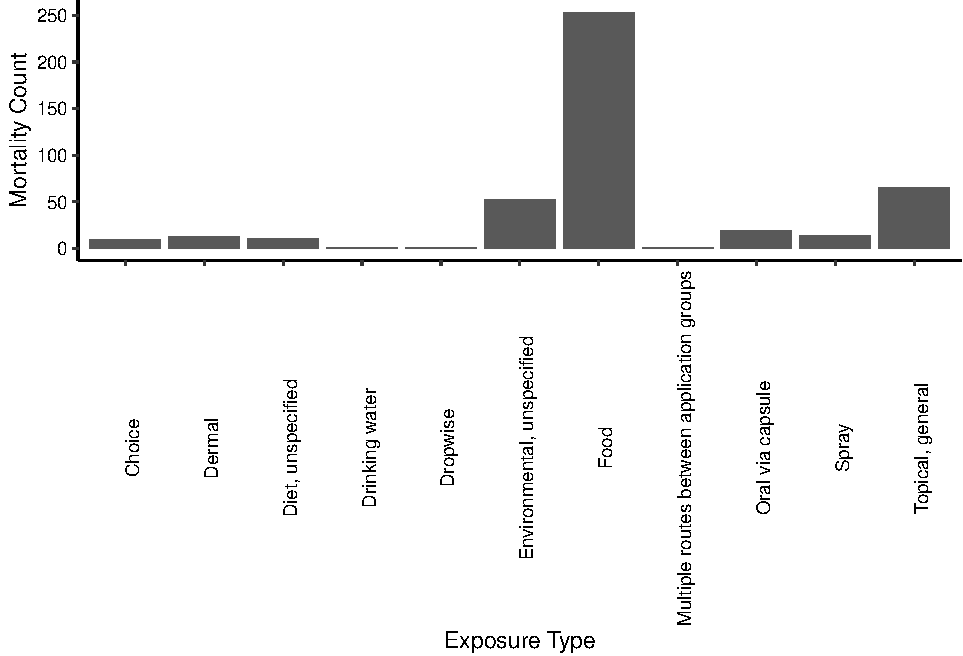
\includegraphics{Project_Template_files/figure-latex/unnamed-chunk-3-1.pdf}
\caption{Bee Mortality}
\end{figure}

\begin{Shaded}
\begin{Highlighting}[]
\NormalTok{ NonBeeMortalityExposure }\OtherTok{\textless{}{-}}\NormalTok{ Mortality }\SpecialCharTok{\%\textgreater{}\%}
  \FunctionTok{filter}\NormalTok{(Species.Common.Name }\SpecialCharTok{!=} \StringTok{"Honey Bee"} \SpecialCharTok{|}\NormalTok{ Species.Common.Name }\SpecialCharTok{!=} \StringTok{"Buff Tailed Bumblebee"} \SpecialCharTok{|}\NormalTok{ Species.Common.Name }\SpecialCharTok{!=} \StringTok{"Carniolan Honey Bee"} \SpecialCharTok{|}\NormalTok{ Species.Common.Name }\SpecialCharTok{!=} \StringTok{"Bumble Bee"} \SpecialCharTok{|}\NormalTok{ Species.Common.Name }\SpecialCharTok{!=} \StringTok{"Italian Honeybee"} \SpecialCharTok{|}\NormalTok{ Species.Common.Name }\SpecialCharTok{!=} \StringTok{"European Dark Bee"} \SpecialCharTok{|}\NormalTok{ Species.Common.Name }\SpecialCharTok{!=} \StringTok{"Buff{-}tailed Bumblebee"} \SpecialCharTok{|}\NormalTok{ Species.Common.Name }\SpecialCharTok{!=}\StringTok{"Stingless Bee"}\NormalTok{)}
 
\NormalTok{ GGPlot\_NonBee\_Mortality\_Exposure }\OtherTok{\textless{}{-}} \FunctionTok{ggplot}\NormalTok{(NonBeeMortalityExposure) }\SpecialCharTok{+}
   \FunctionTok{aes}\NormalTok{(}\AttributeTok{x =}\NormalTok{ Exposure.Type) }\SpecialCharTok{+}
   \FunctionTok{geom\_bar}\NormalTok{() }\SpecialCharTok{+}
   \FunctionTok{ylab}\NormalTok{(}\StringTok{"Mortality Count"}\NormalTok{) }\SpecialCharTok{+}
   \FunctionTok{xlab}\NormalTok{(}\StringTok{"Exposure Type"}\NormalTok{) }\SpecialCharTok{+}
   \FunctionTok{theme}\NormalTok{(}\AttributeTok{axis.text.x =} \FunctionTok{element\_text}\NormalTok{(}\AttributeTok{angle =} \DecValTok{90}\NormalTok{))}
 \FunctionTok{print}\NormalTok{(GGPlot\_HoneyBee\_Mortality\_Exposure)}
\end{Highlighting}
\end{Shaded}

\begin{figure}
\centering
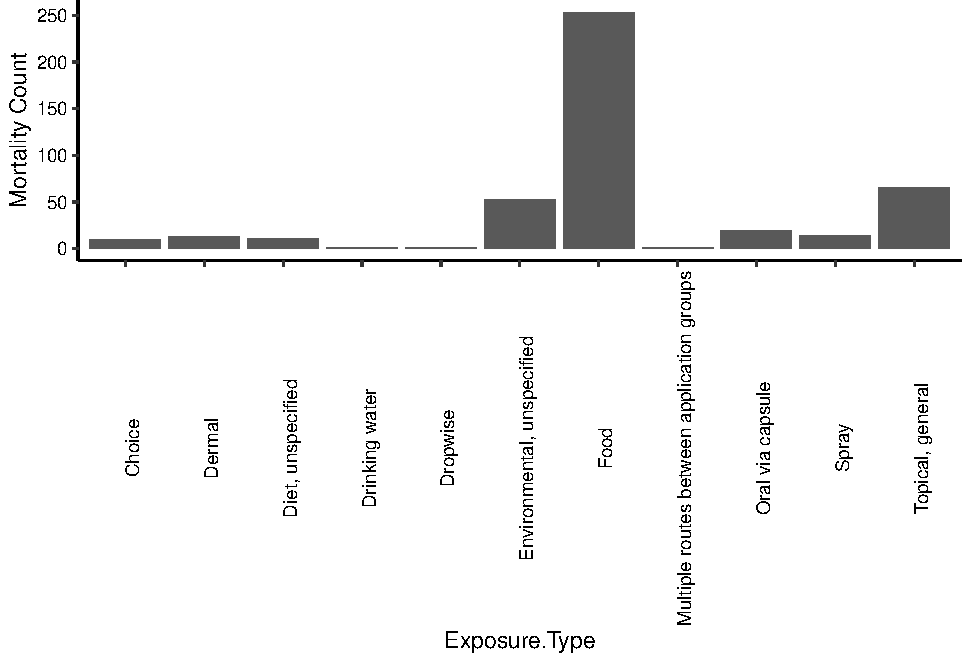
\includegraphics{Project_Template_files/figure-latex/unnamed-chunk-4-1.pdf}
\caption{Non-bee Mortality}
\end{figure}

\newpage

\hypertarget{analysis}{%
\section{Analysis}\label{analysis}}

\hypertarget{question-1-is-there-an-exposure-type-that-has-less-impact-on-bees-than-non-bee-insects}{%
\subsection{Question 1: Is there an exposure type that has less impact
on bees than non-bee
insects?}\label{question-1-is-there-an-exposure-type-that-has-less-impact-on-bees-than-non-bee-insects}}

\hypertarget{question-2-are-there-chemicals-that-have-a-high-mortality-rate-for-non-bee-insects-and-low-rate-for-bees}{%
\subsection{Question 2: Are there chemicals that have a high mortality
rate for non-bee insects and low rate for
bees?}\label{question-2-are-there-chemicals-that-have-a-high-mortality-rate-for-non-bee-insects-and-low-rate-for-bees}}

\newpage

\hypertarget{summary-and-conclusions}{%
\section{Summary and Conclusions}\label{summary-and-conclusions}}

\newpage

\hypertarget{references}{%
\section{References}\label{references}}

\textless add references here if relevant, otherwise delete this
section\textgreater{}

\end{document}
